% Technical report: Solar Filament Segmentation Challenge 2026
% Written for the IEEE conference class. If the competition's Overleaf template differs,
% copy the body (from \begin{abstract} to the bibliography) into it and upload figures/.
\documentclass[conference]{IEEEtran}
\usepackage{graphicx}
\usepackage{booktabs}
\usepackage{amsmath}
\usepackage{url}
\usepackage[hidelinks]{hyperref}
\graphicspath{{figures/}}

\begin{document}

\title{Class-Agnostic Mask R-CNN at Native Resolution for\\Solar Filament Instance Segmentation}

% TODO: confirm name, affiliation, e-mail and Kaggle team name
\author{\IEEEauthorblockN{Sagar Mahadik}
\IEEEauthorblockA{Kaggle team: TODO\\
TODO affiliation\\
TODO e-mail}}

\maketitle

\begin{abstract}
We segment individual solar filaments in GONG full-disk H$\alpha$ images for the
Solar Filament Segmentation Challenge 2026. Our pipeline fine-tunes a COCO-pretrained Mask R-CNN
(ResNet50-FPN) with a single \emph{filament} class on full-resolution $1024\times1024$ crops, runs
it on the native $2048\times2048$ image, fuses horizontal/vertical-flip test-time augmentation at
the instance level, and resolves overlaps by score-ordered painting with thresholds tuned on a
held-out, image-grouped validation split. The final model reaches a validation Panoptic Quality
(PQ) of 0.419 (Dice 0.662), above the 0.34 PQ measured between independent annotators of the same
images, and 0.37 PQ on the public leaderboard. Training takes about
3.7\,h and inference 2.2\,s per image on a 4\,GB consumer GPU (GTX 1650). Code, weights and an
end-to-end notebook are public.
\end{abstract}

\section{Introduction}
Solar filaments are clouds of cool, dense plasma suspended in the corona; on the disk they appear
as dark, elongated, often thin and fragmented structures in H$\alpha$. The challenge asks for one
mask per filament, scored by Panoptic Quality~\cite{kirillov2019panoptic},
\[
\mathrm{PQ}=\frac{\sum_{(p,g)\in TP}\mathrm{IoU}(p,g)}{|TP|+\tfrac12|FP|+\tfrac12|FN|},
\]
where a prediction and a ground-truth (GT) filament match when IoU$>0.5$. PQ therefore rewards
both accurate masks and correct instance separation: splitting one filament into two pieces or
merging neighbours is penalised twice (an FN and one or more FPs). This favours methods that
predict instances directly over semantic segmentation followed by connected components, which tend
to fragment thin filaments. We chose a two-stage instance segmenter and invested in the parts that
matter for PQ at this data scale: native resolution, an honest validation protocol, and
instance-level post-processing.

\section{Data}
The training set (MAGFiLO~\cite{magfilo}) contains 707 unique $2048\times2048$ 8-bit grayscale
images from six GONG sites (Big Bear, Cerro Tololo, Learmonth, Mauna Loa (Mh), El Teide, Udaipur;
102--127 images each). 296 images were annotated by two or three annotators, giving 1154 annotated
samples and 8199 filament polygons (median 7 per sample, median area 1228\,px, 5th--95th
percentile 316--6963\,px). The test set has 180 images.

\textbf{Label noise.} Scoring one annotator's polygons against another's on the same image gives
PQ 0.34 (SQ 0.63, RQ 0.54) over all annotator pairs. Annotators agree on roughly half of the
filaments, and on matched filaments the masks overlap with IoU 0.63 on average. We use this as a
practical reference point for what is achievable.

\textbf{Rules.} Following the competition rules, only the \texttt{segmentation} polygons are used
as training targets. Spines, bounding boxes and chirality classes (\emph{left}, \emph{right},
\emph{unidentifiable}, \emph{ambiguous}) are not used; all filaments form one class.

\textbf{Validation split.} We hold out 15\% of the unique images (106 images, 171 annotated
samples, 1138 filaments), grouped by observation timestamp so an image never appears in both
sets, and stratified by observatory. All annotator versions of a validation image are scored
separately and pooled. The split is fixed (seed 42) and shared by every experiment; all model and
post-processing choices are made on it, never on the leaderboard.

\section{Method}
\subsection{Model}
We use torchvision's Mask R-CNN~\cite{he2017mask} with a ResNet50-FPN backbone pretrained on COCO,
replacing the box and mask predictors with a two-class (background, filament) head. The grayscale
image is repeated over three channels only to match the pretrained stem. Images are never
resized: filaments can be a few pixels wide, and downsampling $2048\to1024$ would halve their
width. Frozen BatchNorm uses $\varepsilon=0$, as in the COCO weights.

\subsection{Training}
Each iteration samples a random $1024\times1024$ crop at native resolution; with probability 0.8
the crop is centred near a randomly chosen filament (with $\pm35\%$ jitter), otherwise uniformly.
Augmentation: horizontal and vertical flips, random $90^\circ$ rotations, and brightness, contrast
and gamma jitter. Instances cropped to fewer than 16 pixels are dropped. We train for 24 epochs
(983 samples per epoch) with SGD (lr 0.005, momentum 0.9, weight decay $10^{-4}$), batch size 1 with
4-step gradient accumulation, 150 warm-up steps followed by cosine decay, and gradient clipping at 10.
Mixed precision was disabled: on the GTX 1650 it produced NaN mask losses and was about 5$\times$
slower than fp32. Training needs 1.9\,GB of GPU memory at 0.52\,s per iteration ($\approx$9\,min per
epoch). Validation PQ is computed every four epochs and the best checkpoint is kept
(Fig.~\ref{fig:curve}).

\begin{figure}[t]
\centering
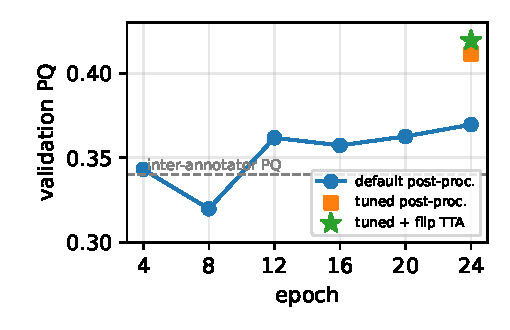
\includegraphics[width=0.92\columnwidth]{val_pq_curve.pdf}
\caption{Validation PQ during training (default post-processing, score threshold 0.5), and the
final model after tuned post-processing and flip TTA.}
\label{fig:curve}
\end{figure}

\subsection{Inference and test-time augmentation}
The model is applied to the full $2048\times2048$ image (2.07\,GB peak GPU memory). With TTA, it is
also applied to the horizontally and vertically flipped image and detections are mapped back.
Detections from the three views are matched greedily by mask IoU$>0.5$; a fused instance takes the
mean mask probability over the views that detected it, and its score is the sum of its scores
divided by the number of views, so detections found in only one view are down-weighted.

\subsection{Post-processing}
Mask R-CNN outputs overlapping, independently scored masks, while PQ needs non-overlapping
instances. Detections are sorted by score and painted onto an occupancy map: each detection keeps
only pixels not yet claimed, and is dropped if its score is below $\tau_s$, if fewer than 50\% of
its binarised pixels survive (a mask-level NMS), or if it is smaller than $A_{\min}$. The score
threshold $\tau_s$, mask threshold $\tau_m$ and $A_{\min}$ are grid-searched on validation
($\tau_s\in[0.3,0.9]$, $\tau_m\in\{0.3,\dots,0.6\}$, $A_{\min}\in\{0,50,150\}$). A high score
threshold is selected ($\tau_s=0.8$ with TTA, 0.85 without; $\tau_m=0.5$; $A_{\min}=0$): under PQ a
false positive costs as much as half a missed filament, so keeping only confident detections pays
off given the label noise. Masks are encoded as COCO RLE with pycocotools for the submission.

\section{Results}
Table~\ref{tab:main} summarises the validation metrics. Dice is the foreground Dice per sample,
computed with \texttt{torchmetrics.segmentation.DiceScore} and averaged (identical to our own
implementation). \emph{1:N} counts GT filaments covered by at least two predictions each lying more
than 50\% inside it (fragmentation); \emph{N:1} counts predictions covering at least two GT filaments
each lying more than 50\% inside it (over-merging). We also ran the organisers' self-evaluation
code unchanged on our validation predictions: it returns the same PQ (0.4193), a mean pairwise IoU
of 0.568 and mean pairwise Dice of 0.702 over the 988 overlapping (GT, prediction) pairs, and, with
its any-overlap definition, 56 GT filaments touched by two or more predictions (1:n) and 40
predictions touching two or more GT filaments (n:1), out of 1138 GT filaments and 1121
predictions.

\begin{table}[t]
\centering
\caption{Validation results (106 images, 171 samples, 1138 GT filaments).}
\label{tab:main}
\setlength{\tabcolsep}{3.5pt}
\begin{tabular}{lcccccc}
\toprule
Configuration & PQ & SQ & RQ & Dice & 1:N & N:1\\
\midrule
Inter-annotator agreement & 0.340 & 0.634 & 0.536 & 0.614 & -- & -- \\
Epoch 4, tuned post-proc. & 0.375 & 0.661 & 0.568 & 0.604 & 45 & 16\\
Epoch 24, default post-proc. & 0.370 & 0.662 & 0.558 & 0.633 & 69 & 32\\
Epoch 24, tuned post-proc. & 0.412 & 0.665 & 0.619 & 0.646 & 34 & 26\\
\quad + hflip TTA & 0.412 & 0.671 & 0.615 & 0.659 & 50 & 25\\
\quad + hflip + vflip TTA (final) & \textbf{0.419} & \textbf{0.671} & \textbf{0.625} & \textbf{0.662} & 43 & 27\\
\bottomrule
\end{tabular}
\end{table}

Tuning the post-processing on validation is the largest single gain (+0.042 PQ), mostly through
recognition quality: false positives fall from 890 to 349. Three-view flip TTA adds a further
+0.008 PQ with consistent gains in SQ (+0.006) and Dice (+0.016), and recovers 40 additional
filaments. On the public leaderboard the epoch-4 and epoch-24 single-view models score 0.33 and
0.36, and the final TTA model 0.37, tracking validation with a stable offset of about $-0.05$. Of the GT filaments,
62\% are matched by some prediction with IoU$>0.5$; matched IoU has a median of 0.68
(Fig.~\ref{fig:dist}).

\begin{figure}[t]
\centering
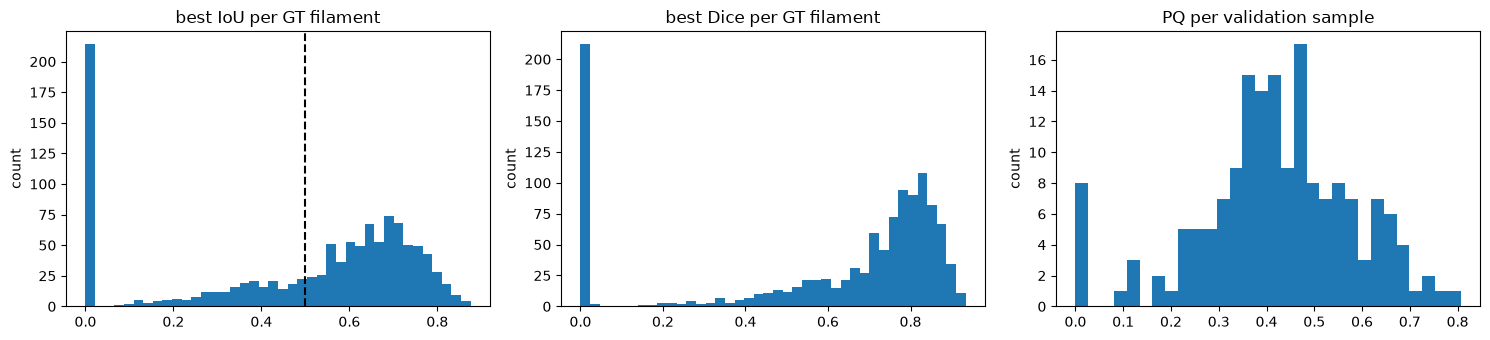
\includegraphics[width=\columnwidth]{distributions.png}
\caption{Validation distributions for the final model: best IoU and Dice per GT filament (dashed:
IoU 0.5 matching threshold) and PQ per validation sample.}
\label{fig:dist}
\end{figure}

\begin{figure}[t]
\centering
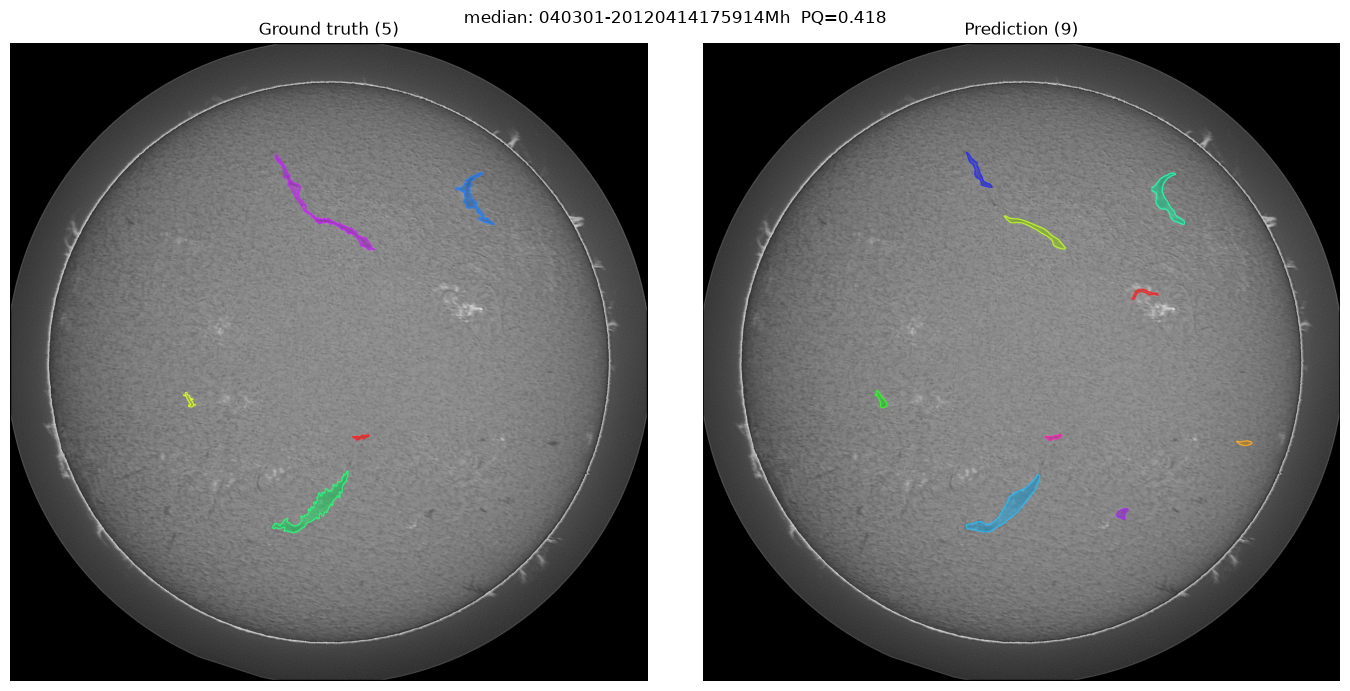
\includegraphics[width=\columnwidth]{val_median.png}\\[2pt]
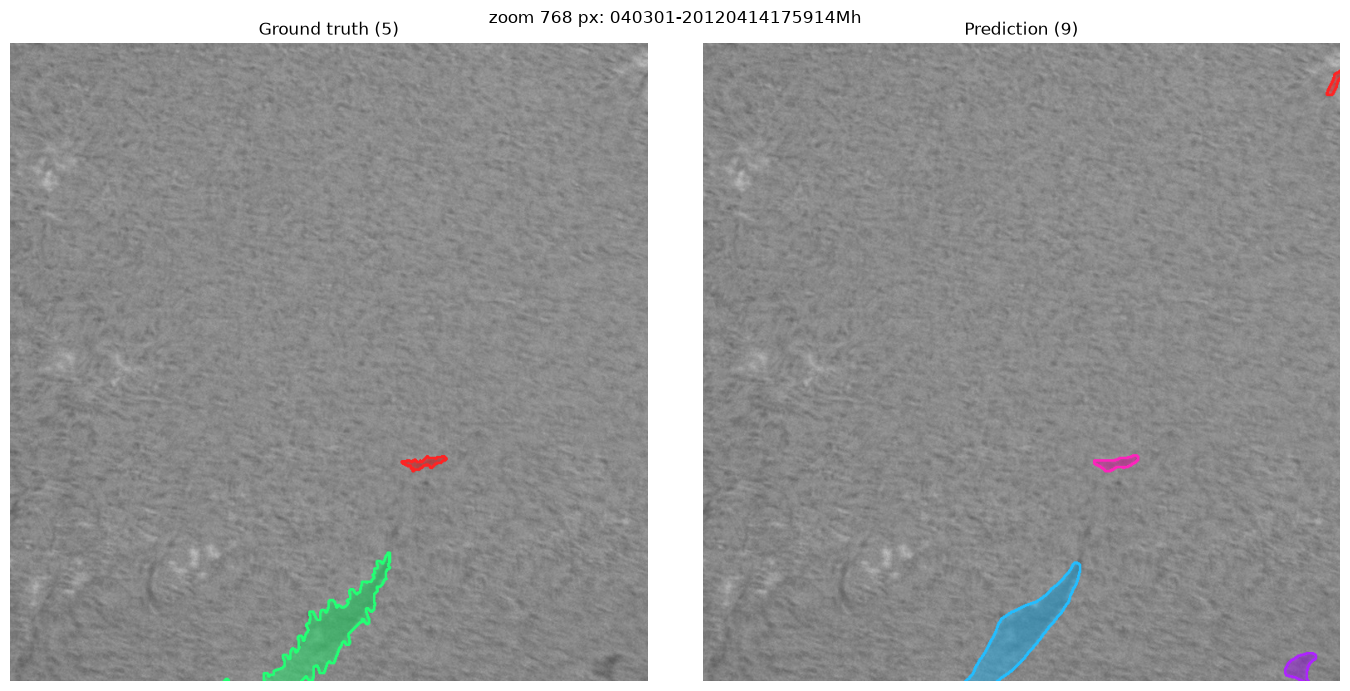
\includegraphics[width=\columnwidth]{val_zoom.png}
\caption{Median validation sample (PQ 0.418). Left: ground truth; right: prediction. Most
filaments are found, with smoother boundaries than the hand-drawn polygons; the long filament at
the top is split into two pieces, and small faint features are detected that the annotator did not
label. Bottom: 768-pixel zoom.}
\label{fig:qual}
\end{figure}

\textbf{Qualitative analysis.} Figure~\ref{fig:qual} shows typical behaviour. Compact and
medium-sized filaments are segmented reliably, with smoother outlines than the annotated polygons,
which limits SQ to about 0.67. The main error modes are (i) long, thin, curved filaments that are
split into several instances or whose faint segments are missed; (ii) small, low-contrast
filaments that the model detects but the annotator did not label, or the reverse, which is the
same ambiguity that limits inter-annotator agreement; and (iii) occasional merging of nearby
filaments.

\textbf{Efficiency.} Training: 24 epochs, about 3.7\,h on a single GTX 1650 (4\,GB), 1.9\,GB peak
memory. Inference on the 180 test images: 1.0\,s per image single-view and 2.2\,s per image with
three-view TTA (fp32, 2.07\,GB peak), plus 5\,s in total for post-processing and RLE encoding. The
model has 44.0\,M parameters and is stored as an 84\,MB fp16 file.

\section{Reproducibility}
The public repository contains all code (\texttt{src/}), the configuration
(\texttt{configs/baseline\_tta.yaml}), the fixed split, the final weights with the tuned
post-processing parameters, \texttt{requirements.txt} with exact versions (Python 3.12, PyTorch
2.14.1, torchvision 0.29.1), and unit tests for the metrics and post-processing. The notebook
\texttt{notebooks/pipeline.ipynb} runs the full pipeline from the committed weights (data and
split, model loading, validation metrics and figures, test inference, CSV writing and format
checks) and reproduces the submitted CSV row for row; setting \texttt{RUN\_TRAINING=True}
retrains from COCO weights. Seeds are fixed and re-seeded every epoch so interrupted runs resume
deterministically from full checkpoints. Weights are saved in fp16 to stay within GitHub's file
size limit; BatchNorm running statistics are kept in fp32, because small variances underflow to
zero in fp16 and, with $\varepsilon=0$, would produce non-finite activations.

\section{Conclusion and future work}
A class-agnostic Mask R-CNN at native resolution, with careful validation and PQ-aware
post-processing, slightly exceeds inter-annotator agreement on this dataset while running on a
4\,GB GPU. The remaining errors are dominated by long, thin filaments and by label ambiguity.
Promising directions are training against all annotators jointly (e.g. soft or consensus
targets), higher-resolution mask heads or contour refinement for thin structures, and ensembles
of models trained with different seeds.

\begin{thebibliography}{9}
\bibitem{kirillov2019panoptic}
A.~Kirillov, K.~He, R.~Girshick, C.~Rother, and P.~Doll\'ar, ``Panoptic segmentation,'' in
\emph{Proc. CVPR}, 2019, pp. 9404--9413.
\bibitem{he2017mask}
K.~He, G.~Gkioxari, P.~Doll\'ar, and R.~Girshick, ``Mask R-CNN,'' in \emph{Proc. ICCV}, 2017,
pp. 2961--2969.
\bibitem{magfilo}
A.~Ahmadzadeh \emph{et al.}, ``MAGFiLO: a large-scale annotated dataset of solar filaments,''
\emph{Scientific Data}, 2024, doi:10.1038/s41597-024-03876-y. % TODO: verify exact title and authors
\end{thebibliography}

\end{document}
